% beautiful title slides in Beamer
% Model 2
% latex-beamer.com

\documentclass[aspectratio=169, compress]{beamer}
\usetheme[
    outer/progressbar=foot, 
    sectionpage=progressbar,
    subsectionpage=progressbar, 
    numbering=counter
]{metropolis}
\setbeamertemplate{subsection page}[numbered]
\setbeamertemplate{subsection in toc}[subsections numbered]
%\setbeamertemplate{frame footer}{\insertsectionhead}
%\setbeamertemplate{progress bar in head}{\insertsectionhead}


\setbeamertemplate{navigation symbols}{}
\setbeamertemplate{caption}[numbered]

\useoutertheme[subsection=false]{miniframes} %<<<<<<<<<<<<<<<<
\setbeamercolor{section in head/foot}{fg=white, bg=mDarkTeal} %<<<<<<<<<<<<<<<<
%\setbeamercolor{subsection in head/foot}{fg=white, bg=mDarkTeal} %<<<<<<<
%\setbeamercolor{title in head/foot}{fg=black, bg=white!50!MSUgreen} %<<<<<<<<<<<<<<<<


\usepackage{appendixnumberbeamer}
\usepackage{booktabs}
\usepackage[scale=2]{ccicons}


\title{Refrigeración en centros de procesamiento de datos}
\date{\today}
\author{Ana Buendía Ruiz-Azuaga \and Andrés Millán Muñoz \and Paula Villanueva Núñez} 
\institute{Universidad de Granada}

\begin{document}
\maketitle

\begin{frame}{Tabla de contenidos}
    \setbeamertemplate{section in toc}[sections numbered]
    \tableofcontents
\end{frame}

\section{¿Por qué es importante la refrigeración?}    % Preliminares 




\section{Sistemas de refrigeración de CPDs}



\subsection{Basados en aire}

\begin{frame}{Free Cooling}
    AAAA
\end{frame}

\begin{frame}{Pasillos calentorros y fríos}
    \begin{figure}
        \begin{center}
            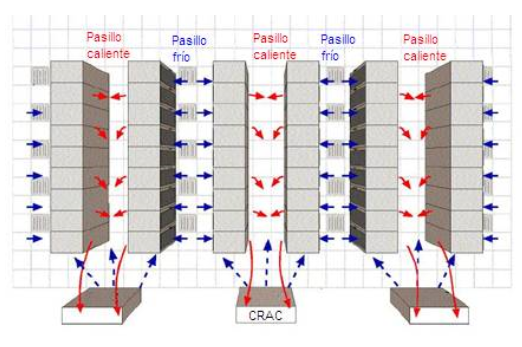
\includegraphics[scale=0.7]{../figures/pasillos}
            \caption{Esquema de los pasillos calientes y fríos. Fuente: \cite{Kelvion}.}
            \label{pasillos}
        \end{center}
    \end{figure}
\end{frame}

\begin{frame}{Confinamiento de zonas}
    AAAA
\end{frame}

\begin{frame}{Refrigeración adiabática}
    AAAA
\end{frame}

\begin{frame}{In-Rack Heat Extraction}
    AAAA
\end{frame}

\begin{frame}{Aire acondicionado para la sala de ordenadores (CRAC)}
    AAAA
\end{frame}

\begin{frame}{Controlador de aire para la sala de ordenadores (CRAH)}
    AAAA
\end{frame}

\begin{frame}{Refrigeración calibrada CVC}
    AAAA
\end{frame}

\begin{frame}{Falsos suelos y techos}
    AAAA
\end{frame}

\begin{frame}{Expansión directa}
    AAAA
\end{frame}



\subsection{Basados en agua}

\begin{frame}{Sistema de agua helada}
    AAAA
\end{frame}

\begin{frame}{Enfriamiento evaporativo}
    AAAA
\end{frame}



\subsection{Basados en inmersión}

\begin{frame}{Cómo funciona inmersión}
    a
\end{frame}

\section{Futuro}

\begin{frame}{Cómo funciona inmersión}
    a
\end{frame}

\section{Soluciones propietarias}

\begin{frame}{Cómo funciona inmersión}
    a
\end{frame}

\section{Conclusiones}

\begin{frame}{Cómo funciona inmersión}
    a
\end{frame}

\end{document}
